% gjilguid2e.tex
% V2.0 released 1998 December 18
% V2.1 released 2003 October 7 -- Gregor Hutton, updated the web address for the style files.

%\documentclass[extra,mreferee]{gji}
\documentclass[extra]{gji}
\usepackage{timet}

%Extra packages
\usepackage{graphicx}

\title[Gravity disturbance or gravity anomaly?]
      {Gravity disturbance or gravity anomaly?}
      
\author[Oliveira Jr, Barbosa and Uieda]
{Vanderlei C. Oliveira Jr$^1$\thanks{Sei la, Nacional, Brazil}, Val\'{e}ria C. F. Barbosa$^1$ and Leonardo Uieda$^2$ \\
	$^1$ Department of Geophysics, Observat\'{o}rio Nacional, Rio de Janeiro, Brazil \\
	$^2$ Department of Geology and Geophysics, University of Hawaii, Manoa, USA
}

\date{Received 2018 Month XX; in original form 2018 Month XX}
\pagerange{\pageref{firstpage}--\pageref{lastpage}}
\volume{XXX}
\pubyear{2018}

%\def\LaTeX{L\kern-.36em\raise.3ex\hbox{{\small A}}\kern-.15em
%    T\kern-.1667em\lower.7ex\hbox{E}\kern-.125emX}
%\def\LATeX{L\kern-.36em\raise.3ex\hbox{{\Large A}}\kern-.15em
%    T\kern-.1667em\lower.7ex\hbox{E}\kern-.125emX}
% Authors with AMS fonts and mssymb.tex can comment out the following
% line to get the correct symbol for Geophysical Journal International.
\let\leqslant=\leq

\newtheorem{theorem}{Theorem}[section]

\begin{document}

\label{firstpage}

\maketitle


\begin{summary}
 Gravity anomalies have long been used by geophysicists for the 
 purpose of determining density distributions in subsurface.
 
 However, gravity anomalies 
 
 In this paper, we discuss the fundamental concepts 
 
 URGENTE: \citep{marussi1974}, \citep{torge2012}, section 4.2.1
\end{summary}

\begin{keywords}
 potential fields -- gravity disturbance -- gravity anomaly -- gravity modeling.
\end{keywords}

\section{Introduction}

The resultant of gravitational force and centrifugal force acting 
on a body at rest on the Earth's surface is called 
\textit{gravity vector} and its intensity is called simply 
\textit{gravity} \citep{hofmann-wellenhof-moritz2005}.
In the case of gravimetry on moving platforms (e.g., airplanes,
helicopters, marine vessels), there are additional
non-gravitational accelerations due to the vehicle motion, 
such as Coriolis acceleration and high-frequency vibrations 
\citep{glennie-etal2000,nabighian-etal2005-grav,baumann-etal2012}.
Geophysicists use gravity for estimating the Earth's 
internal density distribution whereas geodesists use
gravity to estimate the geoid \citep{li2001}.
Hence, geophysicists are usually interested 
in the gravitational component of the observed gravity, 
which is produced by the Earth's internal 
density distribution.
%In applied geophysics, gravity surveys are usually conducted 
%over local or regional areas on the Earth's surface for the purpose of 
%characterizing geological structures located within the
%crust and upper mantle.
%
%Consequently, geophysicists are only interested in the
%particular gravitational component of gravity which 
%is produced by these target geological structures.
The first step of the procedure for isolating this 
gravitational component consists in removing the non-gravitational 
effects due to the vehicle motion and also the time variations 
such as Earth tides, instrumental drift and barometric 
pressure changes, for example.
If these effects are properly removed, the resultant 
gravity data can be considered as the sum of a 
centrifugal component due to the Earth's rotation and
a gravitational component produced by the whole Earth's
internal density distribution.
The isolation of this particular gravitational component 
and its subsequent use for estimating density 
distributions related to geological structures in subsurface 
are the main goals in applied geophysics 
\citep{blakely1996}.

Based on well-established concepts of the literature,
we present a discussion aiming at bringing some
light to the following question: in geophysical applications,
should we use the gravity disturbance or gravity anomaly?
It seems that this theoretical issue has been 
debated within the scientific community from a 
more geodetic than geophysical point of view
\citep{lafehr1991,chapin1996,li2001,fairhead2003,
hackney-featherstone2003,hinze2005}.
Our reasoning suggests that the gravity 
disturbance is more appropriated than gravity anomalies for 
approximating the gravitational effect produced by the Earth's 
internal density distribution.

\section{Normal Earth and normal gravity}


Traditionally, the Earth's gravity field is approximated 
by the gravity field produced by a geocentric and rigid ellipsoid 
of revolution, which has the minor axis $b$ 
coincident with the mean rotating axis of the Earth $Z$, the 
same total mass (including the atmosphere) and also the
same angular velocity of the Earth (Figure \ref{fig:fig1}).
Another characteristic of this model is that its
limiting surface coincides with a particular equipotential 
of its own gravity field.
This model is called as \textit{normal Earth} 
\citep{heiskanen-moritz1967,vanicek1987,hofmann-wellenhof-moritz2005,
torge2012}.


It is worth noting that, although the normal Earth has the
same total mass (including the atmosphere) of the Earth,
its internal density distribution is unknown.


The only condition imposed on its internal density
distribution is that it produces a gravity field
having a particular equipotential which coincides
with its limiting surface.


For convenience, we denote any density distribution 
satisfying this condition as a \textit{normal density distribution}.


Similarly to the gravity vector and gravity, 
the resultant of the virtual 
gravitational and centrifugal forces exerted by the normal
Earth on a body at rest at a point $P$ is called 
\textit{normal gravity vector} and its intensity is called 
simply \textit{normal gravity}.


The normal Earth gives rise to the \textit{geodetic coordinate system}.
In this coordinate system, the position of a point $P$
is defined by the \textit{geometric height} $h$, 
\textit{geodetic latitude}
$\varphi$ and \textit{longitude} $\lambda$ (Figure \ref{fig:fig1}).
Geodetic coordinates $(h, \varphi, \lambda)$ can be easily 
converted into geocentric Cartesian coordinates $(X, Y, Z)$
(Figure \ref{fig:fig1}).


The plane containing the point $P$, the axis $Z$ and
the origin $O$ of this \textit{geocentric Cartesian coordinate system}
is called meridian plane (gray plane in Figure \ref{fig:fig1}).

\begin{acknowledgments}
The authors would like to thank the editor and all the
reviewers for their criticisms and corrections.
\end{acknowledgments}

\bibliographystyle{gji}
\bibliography{bib-file}


\appendix
%\section{For authors}
%
%Table~\ref{authors} is a list of design macros which are unique to GJI. The
%list displays each macro's name and description.
%
%\section{For editors}
%
%The additional features shown in Table~\ref{editors} may be used for
%production purposes.
%
%\bsp % ``This paper has been produced using the Blackwell
%     %   Publishing GJI \LaTeXe\ class file.''

\begin{figure}
%    \vspace{5.5cm}
    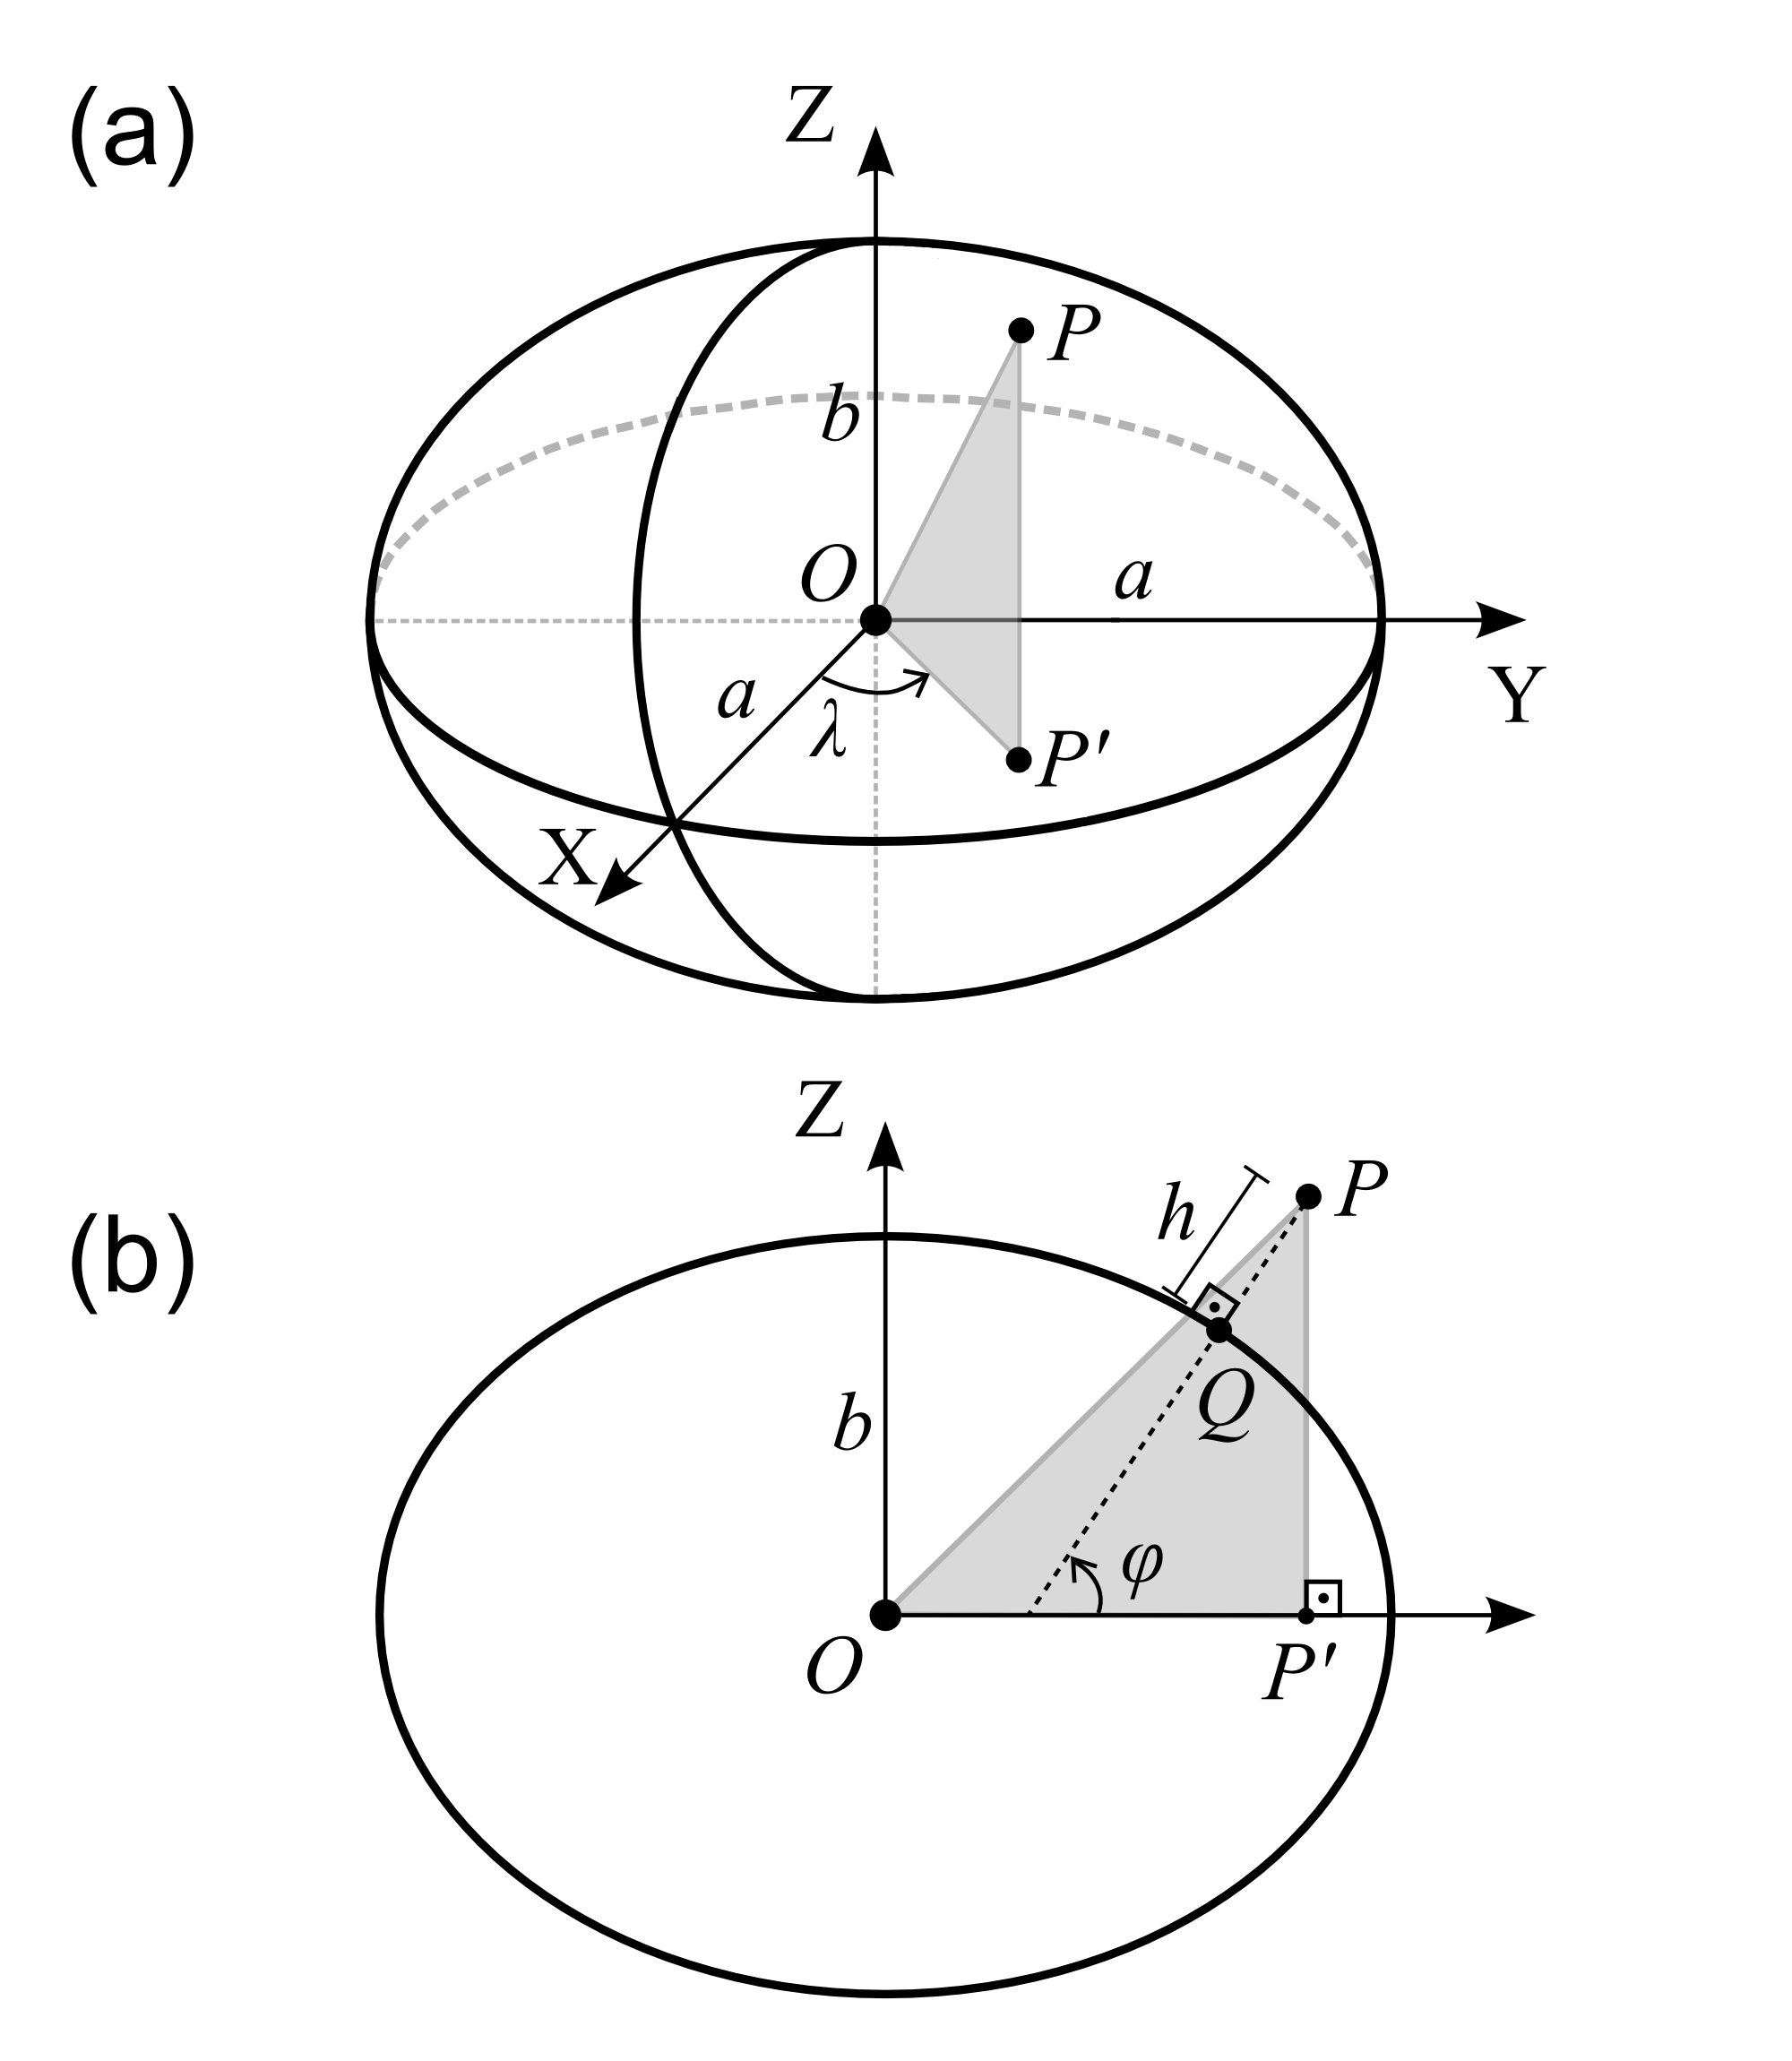
\includegraphics{figures/geodetic_coordinates.png}
    \caption{Schematic representation of the geodetic coordinate
    system defined by an oblate ellipsoid with semi-minor axis $b$, 
    coincident with the mean Earth's rotation axis, and a semi-major
    axis $a$. In this coordinate system, the position of a point is
    determined by the geometric height $h$, the geodetic latitude 
    $\varphi$ and longitude $\lambda$. The Earth's origin is represented 
    by $O$, $P$ represents a point $(h, \varphi, \lambda)$ and 
    $P^{\prime}$ represents the projection of $P$ on the plane $XY$ 
    (Equatorial plane). The plane containing $O$, $P$ and 
    $P^{\prime}$ is represented by the gray triangle in (a) and (b). 
    In (b), the point $Q$ represents the projection of $P$ on the 
    ellipsoid surface.}
  \label{fig:fig1}
\end{figure}

\label{lastpage}


\end{document}